\chapter{Аналитический раздел}
\label{cha:analysis}

Требуется разработать драйвер для графического планшета, позволяющий работать устройству в качестве клавиатуры. В данном разделе рассматриваются методы решения поставленной задачи.

\section{Графический планшет}

Графический планшет -- это устройство для ввода информации, созданной от руки, непосредственно в компьютер. Состоит из пера (стилуса) и плоского планшета, чувствительного к нажатию или близости пера.

Для разработки и тестирования данной работы используется планшет Wacom CTL-671, его изоражение представлено на рисунке \ref{fig:wacom}.

\begin{figure}[H]
    \centering
    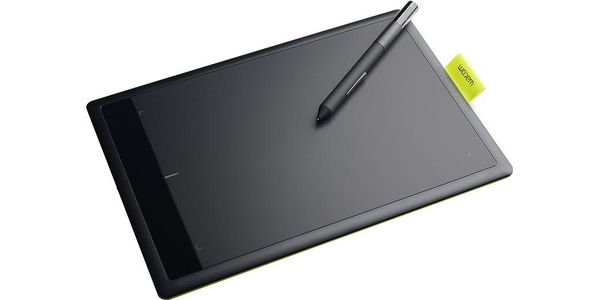
\includegraphics[width=0.8\textwidth]{img/wacom.jpg}
    \caption{Графический планшет Wacom CTL-671}
    \label{fig:wacom}
\end{figure}

\section{Загружаемый модуль ядра}

Загружаемый модуль ядра -- объектный файл, содержащий код, расширяющий возможности ядра операционной системы. Модули используются, чтобы добавить поддержку нового оборудования или файловых систем или для добавления новых системных вызовов. Когда функциональность, предоставляемая модулем, больше не требуется, он может быть выгружен, чтобы освободить память и другие ресурсы.

\subsection{Драйвер устройства}

Драйверы устройств являются одной из разновидностей модулей ядра. Они играют особую роль. Драйверы полностью скрывают детали, касающиеся рабоыт устройства и предоставляют четкий программный интерфейс для работы с аппаратурой. В Unix каждое аппаратное устройство представлено псевдофайлом (файлом устройства) в каталоге /dev. Этот файл обеспечивает средства взаимодействия с аппаратурой.

\section{Подключение графического планшета}

Первой задачей стоит подключение графического планшета для обработки прерываний при нажатии на устройство.

\subsection{Прерывания}

Прерывание -- сигнал к процессору, испускаемый аппаратными средствами или программным обеспечением, и указывающий на событие, которое требует немедленного внимания. Прерывание предупреждает процессор о высокоприоритетном состоянии, требующем прерывания текущего кода, выполняемого процессором. Процессор отвечает, приостанавливая свои текущие действия, сохраняя свое состояние и выполняя функцию, называемую обработчиком прерываний (или подпрограммой обработки прерываний, ISR) для обработки события. Это прерывание является временным, и после завершения обработки обработчика прерывания процессор возобновляет обычную работу. Существует два типа прерываний: аппаратные прерывания и программные прерывания \cite{Interrupts}.

Каждое прерывание имеет свой собственный обработчик прерываний. Количество аппаратных прерываний ограничено числом строк запроса прерывания (IRQ) для процессора, но могут быть сотни различных программных прерываний. Прерывания — это широко используемая техника многозадачности компьютеров, в первую очередь в реальном времени. Такая система называется управляемой прерываниями.

\subsection{Драйвер usb устройства}

Для того, чтобы перехватывать прерывания графического планшета необходимо создать драйвер usb устройства и подключить планшет к нему.

\subsubsection{Структура usb\_driver}

Для создания драйвера usb устройства необходимо использовать структуру usb\_driver \cite{Usb_driver}. 4 главных поля, которые необходимо использовать это: name (имя загружаемого драйвера), probe (указатель на функцию, вызывающуюся при подключении устройства), disconnect (указатель на функцию, вызывающуюся при отключении устройства) и id\_table (список устройств, которые надо автоматически подключать к драйверу, для идентификации устройства используются id поставщика устройства и id самого устройства).

\subsubsection{Работа драйвера usb устройства}

После создания экземляра структуры, представляющей из себя usb драйвер, его необходимо зарегестрировать в системе с помощью системного вызова usb\_register. Если usb драйвер будет успешно зарегестрирован, то он попытается подключить все подходящие устройства, подключенные к системе и незанятые никаким драйвером. Выбор устройств для попытки подключения делается с помощью поля id\_table. Если функция подключения вернет код успешного завершения, то устройство будет подключено к драйверу \cite{Usb_driver}.

\subsubsection{Подключение графического планшета}

Для подключения планшета в функции probe необходимо проделать следующую последовательность действий:

\begin{itemize}
    \item выделить память для экземпляра структуры планшета;
    \item выделить память для устройства ввода;
    \item выделить память для URB (USB Request Block);
    \item получить свободный путь в файловой системе для устройства ввода;
    \item связать прерывание устройства с функцией;
    \item зарегистрировать устройство.
\end{itemize}

\subsection{Многозадачность для прерываний}

Чтобы сократить время выполнения обработчиков прерываний обработчики медленных аппаратных прерываний делятся на две части, которые традиционно называются верхняя (top) и нижняя (bottom) половины (half). Верхними половинами остаются обработчики, устанавливаемы функцией request\_irq() на определенных IRQ. Выполнение нижних половин инициируется верхними половинами, т.е. обработчиками прерываний \cite{BottomHalf}.

В ОС Linux имеется три типа нижних половин (bottom half) \cite{BottomHalf}:

\begin{itemize}
    \item softirq -- отложенные прерывания;
    \item tascklet -- тасклеты;
    \item workqueue -- очереди работ.
\end{itemize}

Для обработки прерываний испольуют тасклеты и очереди работ. Рассмотрим данные методы.

\subsubsection{Тасклеты}

Тасклеты -- это механизм обработки нижних половин, построенный на основе механизма отложенных прерываний \cite{BottomHalf}.

Тасклеты описываются следующей структурой, описанной на листинге \ref{lst:tasklet} \cite{Tasklets}.

\begin{lstlisting}[language=c,caption=Структура tasklet,label=lst:tasklet]
struct tasklet_struct
{
    struct tasklet_struct *next;
    unsigned long state;
    atomic_t count;
    void (*func)(unsigned long);
    unsigned long data;
};
\end{lstlisting}

В данной структуре имеются поля \cite{Tasklets}:

\begin{itemize}
    \item next -- указатель на следюущий тасклет в списке;
    \item state -- состояние тасклета;
    \item func -- функция обработчик тасклета;
    \item data -- аргумент функции обработчика тасклета.
\end{itemize}

Когда tasklet запланирован, он добавляется в очередь. Пока он находится в этом состоянии, запланировать его еще раз не получится -- в этом случае просто ничего не произойдет. Tasklet не может находиться сразу в нескольких местах в очереди на планирование, которая организуется через поле next структуры tasklet\_struct. После того, как тасклет был запланирован, он выполнится один раз \cite{Tasklets}.

\subsubsection{Очереди работ}

Очередь работ является еще одной концепцией для обработки отложенных функций. Функции рабочих очередей выполняются в контексте процесса ядра. Это означает, что функции очереди задач не должны быть атомарными, как функции тасклета. Подсистема рабочей очереди представляет собой интерфейс для создания потоков ядра для обработки работы (work), которая ставится в очередь. Такие потоки ядра называются рабочими потоками. Рабочая очередь поддерживается типом struct work\_struct, описанным на листинге \ref{lst:work_struct} \cite{WorkQueue}.

\begin{lstlisting}[language=c,caption=Структура work\_struct,label=lst:work_struct]
struct work_struct
{
    atomic_long_t data;
    struct list_head entry;
    work_func_t func;
# ifdef CONFIG_LOCKDEP
    struct lockdep_map lockdep_map;
# endif
};
\end{lstlisting}

Очередь работ создается функцией:

\begin{lstlisting}[language=c]
int create_workqueue(char *name, unsigned int flags, int max_active);
\end{lstlisting}

\begin{itemize}
    \item name -- имя очереди, но в отличие от старых реализаций потоков с этим именем не создается;
    \item flags -- флаги определяют как очередь работ будет выполняться;
    \item max\_active -- ограничивает число задач из данной очереди, которые могут одновременно выполняться на одном CPU.
\end{itemize}

Для того, чтобы поместить задачу в очередь работ надо заполнить (инициализировать) структуру work\_struct.

После того, как работа была создана, следующим шагом будет помещение этой структуры в очередь работ. Это можно сделать несколькими способами. Во-первых, просто добавить работу (объект work) в очередь работ с помощью функции queue\_work (которая назначает работу текущему процессору). Можно с помощью функции queue\_work\_on указать процессор, на котором будет выполняться обработчик.
Две дополнительные функции обеспечивают те же функции для отложенной работы (в которой инкапсулирована структура work\_struct и таймер, определяющий задержку): queue\_delayed\_work, queue\_delayed\_work\_on \cite{WorkQueue}.

Кроме того, можно использовать глобальное ядро -- глобальную очередь работ с четырьмя функциями, которые работают с этой очередью работ. Эти функции имитируют предыдущие функции, за исключением лишь того, что не нужно определять структуру очереди работ \cite{WorkQueue}.

\section{Работа клавиатуры}

Для эмуляции работы клавиатуры необходимо вызывать нажатия клавиш после обработки прерываний графического планшета.

\subsection{Подсистема ввода/вывода}

Подсистема ввода/вывода выполняет запросы файловой подсистемы и подсистемы управления процессами для доступа к периферийным устройствам (дискам, магнитным лентам, терминалам и т.д.). Она обеспечивает необходимую буферизацию данных и взаимодействует с драйверами устройств — специальными модулями ядра, непосредственно обслуживающими внешние устройства \cite{Subsystem}.

Подсистемой ввода/вывода поддерживаются три вида устройств:

\begin{itemize}
    \item символьные устройства для поддержки последовательных устройств;
    \item блочные устройства для поддержки устройств с произвольным доступом, блочные устройства имеют важное значение для реализации файловых систем;
    \item сетевые устройства, которые поддерживают широкий спектр устройств на канальном уровне.
\end{itemize}

Для использования подсистемы ввода/вывода используется структура input\_dev \cite{Input_dev}. Чтобы инициализировать эту структуру используется функция set\_bit, которая принимает два аргумента: бит, который устанавливается, и адрес, куда этот бит устанавливать \cite{Setbit}.

\subsubsection{Установка событий}

Для установки типа события, которое будет вызываться необходимо установить бит EV\_KEY \cite{EVkey} в поле evbit в структуре input\_dev \cite{Input_dev}. После установки бита события устанавливаются биты клавиш, которые будут вызываться, например, KEY\_0 (клавиша с цифрой 0), KEY\_Z (клавиша с буквой z) и KEY\_CAPSLOCK (клавиша CapsLock).

\subsubsection{Вызов событий}

Для вызова событий, связанных с клавишами используется системный вызов input\_report\_key \cite{Input_report_key}, который принимает устройство ввода (структура input\_dev), клавишу, на которую вызывается событие, и код события. В данной работе необходимы два кода событий: 1 -- кнопка зажата, 0 -- кнопка отжата.

\section{Вывод}

Таким образом были рассмотрены методы решения задачи разработки драйвера нулевого уровня для использования графического планшета в качестве клавиатуры.
